\documentclass[preprint,12pt]{elsarticle}
\usepackage{etoolbox}
\makeatletter
\patchcmd{\ps@pprintTitle}{\footnotesize\itshape
       Preprint submitted to \ifx\@journal\@empty Elsevier
       \else\@journal\fi\hfill\today}{\relax}{}{}
\makeatother

%% Use the option review to obtain double line spacing
%% \documentclass[preprint,review,12pt]{elsarticle}

%% Use the options 1p,twocolumn; 3p; 3p,twocolumn; 5p; or 5p,twocolumn
%% for a journal layout:
%% \documentclass[final,1p,times]{elsarticle}
%% \documentclass[final,1p,times,twocolumn]{elsarticle}
%% \documentclass[final,3p,times]{elsarticle}
%% \documentclass[final,3p,times,twocolumn]{elsarticle}
%% \documentclass[final,5p,times]{elsarticle}
%% \documentclass[final,5p,times,twocolumn]{elsarticle}

%% The graphicx package provides the includegraphics command.
\usepackage{graphicx}
%% The amssymb package provides various useful mathematical symbols
\usepackage{amssymb}
%% The amsthm package provides extended theorem environments
%% \usepackage{amsthm}

%% The lineno packages adds line numbers. Start line numbering with
%% \begin{linenumbers}, end it with \end{linenumbers}. Or switch it on
%% for the whole article with \linenumbers after \end{frontmatter}.
\usepackage{lineno}
\usepackage{url}
\bibliographystyle{unsrt}

%% natbib.sty is loaded by default. However, natbib options can be
%% provided with \biboptions{...} command. Following options are
%% valid:

%%   round  -  round parentheses are used (default)
%%   square -  square brackets are used   [option]
%%   curly  -  curly braces are used      {option}
%%   angle  -  angle brackets are used    <option>
%%   semicolon  -  multiple citations separated by semi-colon
%%   colon  - same as semicolon, an earlier confusion
%%   comma  -  separated by comma
%%   numbers-  selects numerical citations
%%   super  -  numerical citations as superscripts
%%   sort   -  sorts multiple citations according to order in ref. list
%%   sort&compress   -  like sort, but also compresses numerical citations
%%   compress - compresses without sorting
%%
%% \biboptions{comma,round}

% \biboptions{}

\begin{document}

\begin{frontmatter}

%% Title, authors and addresses

\title{Picolo: Fast, Decentralized Globally Distributed Database Network\tnoteref{title1}}
\tnotetext[title1]{Work in progress, Version 0.1 Draft.}

\author{Adi Kancherla, Arunesh Mishra\corref{auth1}}
\cortext[auth1]{Email: adi,arunesh@picolo.network}
\address{San Francisco, California}

%% use the tnoteref command within \title for footnotes;
%% use the tnotetext command for the associated footnote;
%% use the fnref command within \author or \address for footnotes;
%% use the fntext command for the associated footnote;
%% use the corref command within \author for corresponding author footnotes;
%% use the cortext command for the associated footnote;
%% use the ead command for the email address,
%% and the form \ead[url] for the home page:
%%
%% \title{Title\tnoteref{label1}}
%% \tnotetext[label1]{}
%% \author{Name\corref{cor1}\fnref{label2}}
%% \ead{email address}
%% \ead[url]{home page}
%% \fntext[label2]{}
%% \cortext[cor1]{}
%% \address{Address\fnref{label3}}
%% \fntext[label3]{}


%% use optional labels to link authors explicitly to addresses:
%% \author[label1,label2]{<author name>}
%% \address[label1]{<address>}
%% \address[label2]{<address>}

\begin{abstract}
%% Text of abstract
Picolo is a fast, scalable, verifiable, fully-decentralized, globally distributed transaction oriented database for
blockchain-based Applications. Picolo uses a probabilistic replication framework on top of DHTs to achieve a O(1)
lookup latency for most queries. Its the first and so-far only system of its kind to distribute data at a global
scale will full-decentralization and externally-consistent distributed transactions.

\begin{itemize}
    \item Allows for verifiable transaction logs.
    \item Token economics that gamify honest participation from nodes over malicious intent.
\end{itemize}
\end{abstract}

\begin{keyword}
Decentralization \sep Blockchain \sep Crypto economics \sep Database \sep Distributed \sep SQL
%% keywords here, in the form: keyword \sep keyword

%% MSC codes here, in the form: \MSC code \sep code
%% or \MSC[2008] code \sep code (2000 is the default)

\end{keyword}

\end{frontmatter}
%-----------------------------------------------------------------------------
%  INTRODUCTION
%-----------------------------------------------------------------------------
\section{Introduction}\label{Sect:Introduction}


    \begin{itemize}
        \item What are Dapps. Dapps will grow, but need to store data.
        \item Solutions today provide file storage semantics which might not work for all application types.
        \item Introduce the database problem on the blockchain. What are the requirements for a decentralized database.
        \item Overview of current approaches and limitations (details in the Background and Related work section).
    \end{itemize}


\subsection{Picolo's Features}
\begin{itemize}
    \item Network layer Scales with O(log N) overhead for N nodes.
    \item Network lookup using O(1) amortized lookup cost for DHT.
    \item Horizontally scalable 
    \item Automated data sharding
    \item Transactions can be applied across rows, columns and tables across machines
    \item Client controlled replication and data placement
    \item Synchronous replication and external consistency, the strongest form of consistency any database can support
    \item SQL like interface
    \item Supports storage of typed data
    \item Supports semi-relational structure for tables
    \item Configurable backups and restore mechanisms
    \item Verifiable legder for transactions.
\end{itemize}

%-----------------------------------------------------------------------------
%  BACKGROUND SECTION
%-----------------------------------------------------------------------------
%-----------------------------------------------------------------------------
%  BACKGROUND SECTION
%-----------------------------------------------------------------------------
\section{Related Work}
There have been attempts in the academia at building peer-to-peer data management systems (PDMS). PeerDB \cite{PeerDB} pioneered a full-fledged data management system that supports fine-grain content-based searching on a distributed network of nodes with heterogeneous schemas. It proposed a "code goes to data" paradigm where mobile agents are employed to perform query processing at a peer node in order to reduce network bandwidth. PIER \cite{PIER} provides a relational data model and query operators on top of any distributed storage system. It embraces the notion of \textit{data independence} and only concerns itself with query processing. It does not provide any sort of replication or ACID guarantees of a database and does not maintain any indexes of its own. Piazza \cite{Piazza} describes a system where peers have pairwise schema mappings between heterogeneous schemas and how these can be transitively extended to answer queries from peers separated by more than one edge. Queries are reformulated at each peer to match the local schema before execution. While this approach works well for a few reformulations, a large number of them may result in information loss or returning of irrelevant results.
\newline\newline


In the blockchain space, there are a few projects tackling the decentralized storage problem. Filecoin \cite{Filecoin}
adds an incentive layer on top of widely used IPFS \cite{ipfs} - a p2p file sharing system. It pays miners for
contributing disk space and network bandwidth to the filecoin system. Storj \cite{Storj} and Sia \cite{Sia} are two
similar projects that offer decentralized file storage systems for end users wanting to store files on more resilient,
secure and censorship resistant networks. While these networks are great for storing large unstructured files like
images, videos, documents etc they are not suitable for storing structured data and do not support complex queries
beyond simple keyword search.

    \begin{itemize}
        \item Bluezelle, fluence, pepperdb
    \end{itemize}




%-----------------------------------------------------------------------------
%  OVERALL DESIGN SECTION
%-----------------------------------------------------------------------------
\section{Overall Design}

    \begin{itemize}
        \item Overall Picolo architecture.
        \item Token economics.
    \end{itemize}




%-----------------------------------------------------------------------------
%  NETWORK SUB-SYSTEM SECTION
%-----------------------------------------------------------------------------
\section{Network Subsystem} 

The network layer is a fully decentralized, peer-peer overlay routing layer among the nodes participating in the Picolo
database network. The most important goal of the network layer is to help locate content as efficiently and quickly as
possible while surviving certain kinds of failure or malicious intent. Peer-peer networking literature refers to this
functionality as Decentralized Object Location and Routing (DOLR) \cite{dolr2003}. The network layer focuses on routing
messages, such as database queries, read/write requests or other management functions to the respective nodes which can
satisfy them. 

The overlay layer can be implemented on top of any datagram network protocol such as UDP or IP. Specifically on the
Internet, we realize its implemented on IP or IPv6 protocols.  The peer-to-peer overlay routing infrastructure offers
efficient, scalable, location-independent routing of messages directly to nearby copies of an object or service using
only localized resources \cite{tapestry2004}. We use the word object to loosely refer to content such as Tables, Shards,
Metadatd and such, that is, any content that is content-addressable and needs to be part of the lookup layer.  Location
independent routing refers to a class of techniques for locating objects based on content rather than their location,
while attempting to find the shortest path possible to reach such objects. Picolo's design offers the following
properties which are required of any high performance p2p overlay-based lookup layer:

\begin{itemize}
    \item {\em Determinstic Node Mapping}: Picolo is able to locate objects anywhere in the network. That is, there
        should be no object in the network that cannot be accessed using the lookup layer.
    \item {\em Low routing inefficiency}: Routes should have low {\em stretch}. Stretch is the ratio between (network
        level) distance traveled by a query to an object and the minimal network distance from the query to the object.
        Optimal solution would be to always send the query to the nearest copy possible.
    \item {\em Balanced load}: The load should be evenly distributed across the nodes in the network, thus, reducing
        hotspots.
    \item {\em Dynamic membership}: THe system allows arrival and departure of nodes while maintaining functionality.
\end{itemize}

-- Self-repairing.
-- Soft-state based routing.

\subsection{Background}

In this Section, we provide a brief overview of peer-peer systems both in the research and product community that have
influenced the literature over the last 20 years.

Napster \cite{Napster} was one of the first popular service that provided much of the original inspiration for peer-peer
systems although its database was centralized.  DNS is an example of a widely deployed distributed and largely
decentralized key-value database that powers every lookup and interaction on the Internet \cite{Mockapetris_1988}. DNS
relies on special root servers to bootstrap the lookup protocol. The Freenet \cite{freenet_thesis, Clarke_2001} and the
Gnutella \cite{Gnutella} p2p systems were popular in the previous decade for file sharing. Both systems were designed
for sharing of large files over a longer duration of time. Content reliabilty including lookup reliability and network
latency goals were necessary in this enviroment. 

The second generation of peer-peer systems include research driven projects such as Chord \cite{Stoica_2001}, Content
Addressable Network (CAN)
\cite{Ratnasamy_2001}, Pastry \cite{Rowstron_2001}, Tapestry \cite{tapestry2004} and
Kademlia. Chord along with CAN, Tapestry and Pastry developed the concept of distributed hash tables (DHTs) as a
fundamental mechanism for content-based addressing. They built over the scalability and self-organizing properties of
both FreeNet and Gnutella by providing a definite answer to a lookup query in a bounded number of network hops. In fact,
these protocols are able to locate content within \( O(log N) \) where \(N\) is the number of nodes in the system. From
an 
API perspective, these overlays provide a key-based routing (KBR) interface that supports deterministic routing of
messages to a live node that has the responsiblity for the "value" corresponding to the given key. These systems also
support high level APIs such as Dynamic Object Location and Routing (DOLR) \cite{dolr2003}. Most DHT's use the concept
of consistent hashing to distribute the load evenly among the nodes.

{\em Consistent hashing:}
Typical hashing based schemes do a good job of spreading load through a known, fixed collection of servers. Since the
Blockchain consists of nodes on the Internet which can appear and disappear based on incentives and other criteria, our
assumption is that machines come and go as they crash or are brought into the network. Also,
the information about what nodes are functional propagates slowly through the
network, so that clients may have incompatible “views” of which nodes are available to replicate data. (Note that a
node can also be a client). This makes standard hashing useless since it relies on clients agreeing on which nodes are responsible for serving a particular
page.

Like most hashing schemes, consistent hashing assigns a set of items to buckets so that
each bin receives roughly the same number of items.  Unlike standard hashing schemes, a small change in the bucket set
does not induce a total remapping of items to buckets. In addition, hashing items into slightly different sets of
buckets gives only slightly different assignments of items to buckets. 

Chord uses such hash functions to map nodes and content uniformly to a circular 160-bit
namespace. Chord improves the scalability of consistent hashing by removing the requirement that every node knows about
every other node. Each node only maintains about \(O (log N) \) state information about other nodes in an \( N \) node
network. When nodes join or leave, they require \( O(log^2 N) \) messages to keep the network updated.

CAN routes messages in a {\em d}-dimensional space where each node maintains a routing table with \(O(d)\) entries and
any node can be reached in \(O(dN^{1/d})\) routing hops. CAN's routing table does not grow with network size, but the
number of routing hops grows faster than \(log N\).

When compared to Chord and CAN, Pastry and Tapestry take network distances into account when constructing overlay
topologies. While Chord and CAN use shortest overlay hops and other runtime heuristics, both Tapestry and Pastry
construct locally optimal routing tables to reduce any routing inefficiencies. 

Pastry and Tapestry share some similarities to the work by Plaxton et al \cite{Plaxton_1997} and to the routing layer in
the Landmark hierarchy \cite{Tsuchiya_1988}. The approach consists of routing based on address prefixes or otherwise
called prefix-based routing. However, both Pastry and Tapestry include an ability to self-organize the network structure
and achieve network locality in content mapping which also lends support for replication.
In addition, Tapestry also allows some application-based locality management by "publishing" location pointers
throughout the network for efficiently locating content and services.

Kademlia \cite{kademlia} is another p2p DHT-based routing system that uses prefix-based routing by arranging 160-bit IDs
(node IDs and content IDs) in a binary tree style data-structure for efficient routing. It uses an XOR-based distance
metric for building the routing table and for the routing algorithm itself. In terms of its performance and other
features, it is very similar to the above systems such as Chord, CAN, Pastry and Tapestry, but it offers simplicity in
its routing and lookup algorithms which make it attrative for implementation. IPFS \cite{ipfs} uses a version of
Kademlia for locating files for decentralized applications.

Other notable systems include Viceroy \cite{viceroy} which provides logarithmic hops through nodes with constant degree
routing tables. SkipNet \cite{skipnet} uses a multidimensional skip-list data structure to support overlay routing,
maintaining both a DNS-based namesapce for operational locality and a randomized namespace for network locality. Other
overlay proposals such as Koorde \cite{koorde} and Naor et al \cite{simple_hash} attain lower bounds on local routing
state but oversimplify some of the other features. 

The third generation of P2P research includes building applications on top of these DHT systems, validating them as
novel infrastructures or tuning them for specific use cases. For example, applications such as PAST \cite{past} and
SCRIBE \cite{scribe} are built on top of Pastry. Decentralized file storage application project OceanStore \cite{oceanstore} was built
on top of Tapestry, while CFS \cite{cfs} was build on top of Chord. FarSite \cite{farsite} uses a conventional
distributed directory service and could be built on top of Pastry. Another example of an overlay network is the Overcast
System \cite{overcast}, which provides reliable single-source multicast streams.

\subsection{Design of the Picolo overlay network}

The Picolo overlay network consists of a p2p DHT based lookup for mapping key to objects, content or services. There is a caching layer that allows for frequenly used items to be propagated closer to the demand endpoints in the network including ability to replicate as needed.

\subsubsection{Picolo namespace} 
1. Nodes and content map to a single 256-bit space. We can use existing hash functions such as SHA-256 for this purpose.

This space can be segregaged using a namespace identifier, which allows multiple such "naming layers" to co-exist. For example, one way to assign naming layers could be based on a per-application type.

For the rest of this section, the discussion gets isolated to within a single naming layer.

\subsubsection{Core API}
Picolo's network layer supports an API similar to a standard p2p overlay network, for a detailed discussion refer
\cite{dolr2003}. The primary goal of the API is to publish and locate objects or service identifiers within a given
namespace. All operations that occur in a namespace can be replicated across namespaces as needed.

Currenlty, we support the following API methods in a decentralized manner:
\begin{itemize}
    \item Publish()
    \item Unpublish()
    \item Lookup()
    \item RemoteCall()
\end{itemize}

\subsubsection{Routing and Lookup}

\begin{itemize}
    \item Lookup using a prefix-based DHT. 
    \item Routing table description.
    \item Lookup algorithm.
    \item Caching links for faster lookup. 
\end{itemize}

\subsection{Node Dynamics}

Failures, node departures, node additions.

\subsection{Replication and caching}
Beehive stuff for O(1) lookups for power law queries

Structured peer-peer distributed hash tables can implement lookups in \( O(log N)\) hops. Since each hop could add between 100-500
ms of latency, for a network of 10K to 100K nodes this computes to about 4-5 seconds for a lookup (or more). Thus, we
require a caching and replication strategy to reduce this cost especially for popular items. The discussion in this
Section applies to any content or service thats is made available through the p2p system and thus extends beyond the
Database as a blockchain service provided by Picolo.

There has been significant prior work on caching and replicating strategies for peer-peer overlay networks. Methods such
as Beehive \cite{beehive} provide a closed-form replication algorithm based on a derived equation that guarantees
\(O(1)\) lookup but require full knowledge of the network, such as number of nodes and popularity values for each data
item. While this system might be good for analysis and benchmark purposes, its implementation is not pratical for
Picolo. Kelips \cite{kelips} is a probabilistic algorithm that also provides \(O(1)\) lookup performance (in the
expected case) by dividing the network into \(O(\sqrt(N))\) affinity groups each of \(\sqrt(N)\) size. They use the
gossip protocol to replicate content to all nodes within an affinity group. Work by Gupta et al \cite{one_hop_lookup}
explore the tradeoff between routing table size and lookup latency. They offer a guaranteed \(O(1)\) lookup by
maintaining routes to each and every node in the network. Farsite \cite{farsite} provides a better ttradeoff by using
routing tables of \(O(dn^{1/3})\) size to route within \(O(d)\) hops.

Other peer-peer applications such as PAST \cite{past} and CFS \cite{cfs} use fixed size caches on intermediate nodes to
cache the objects being queried. While they are unable to provide closed-form analytic bounds on query time, their
average case performance is reasonably good.

We draw on the above literature to find the right balance between routing table size, cache and replication storage at
nodes versus lookup latency. The strategy presented in this Section achieves \(O(1)\) lookup on average for networks with standard node
and popularity dynamics. In other words, we allow for node joins, failures, unexpected departures (including malicious
intent) along with changes in service or object popularity. We also allow for "flash crowds", that is, an item, object
or service (such as a table-shard, or certain rows in a table) can quickly gain popularity (as given by standard
Internet virality models \cite{virality_model}).

\begin{itemize}
    \item A node caches or replicates an item with a probability that is proportional to the number of queries it is
        expected to get for that item in the upcoming time interval T.
    \item The difference between a cache and a replica is application specific. For the Database application that the
        network layer hosts, it depends on whether a particular table or a shard is allowed to have write permissions on
        the replica.
    \item When a node caches or replicates an item, it affects the probabilitic demand distribution for the item at
        nodes that are on the routing path which would have gotten the request has this item not been cached.
    \item Thus, by repeating this algorith iteratively, it would converge to the best caching pattern which would reduce
        lookup times with high probability for all items on the network.
\end{itemize}

\subsection{P2P Connectivity protocol}

When a Picolo node starts for the first time (fresh install), it will query a set of "root" servers, similar to the DNS
architecture of the Internet which is one of the largest decentralized lookup databases in the world \cite{icann_root}. 
These root servers populate the nodes with a list of neighboring nodes and content to bootstrap with.

The nodes use QUIC for server-server connections. QUIC primer. Why QUIC ?

Certain network configuations might not allow for QUIC, such as due to firewalls. In such cases, we will use the SPDY
protocol which offers multi-session transport over the HTTPS ports which every firewall should support.

STUN/NAT traversals and proxies.

\subsection{Cryptoeconomics and Byzantine behavior}
How will malicious nodes affect the system and how to mitigate/prevent/recover. Do nodes have incentive to participate in network discovery

\subsection{Analytics and Debug/Fault diagnosis}



%-----------------------------------------------------------------------------
%  DATABASE SUB-SYSTEM SECTION
%-----------------------------------------------------------------------------
\section{Database Subsystem}
In this section, we discuss core database concepts like byzantine paxos, role of timestamps in achieving external consistency, distributed transactions and sharding. Concepts that are most new to a database network built for the  decentralized world like distributed query processing, dynamic clustering, data sovereignty and decentralized fine-grained access control are presented.

\subsection{Consensus, replication \& sharding} \label{sec:paxos}
All data on \textsf{Picolo} is replicated for durability and high availability. Storage consumers have the option of choosing a replication factor that suits their needs. They can also choose where to locate their data based on where their users are located to achieve better latency or to comply with regulations like GDPR. This data locality can easily be achieved by instructing the network layer to only allow replicas that belong to a geographic region to join the replica group. Consensus is achieved amongst replicas by a running a variant of paxos that is tolerant to byzantine faults.
 \subsubsection{Paxos based replication}
 We modify the algorithms in \cite{byzantine_paxos} to make the leader election more frequent and add a slashing condition that punishes byzantine behavior. There are two roles that each replica can take: \textsf{proposer} and \textsf{acceptor}. Proposers initiate changes to the state by proposing new commands to be appended to a \textsf{sequence} from which the replica state is generated and acceptors vote on which sequence to accept. The system moves through different \textsf{views}. A view can be thought of as a discrete time period (in the order of minutes) with a monotonically increasing view number $\textsf{view}_\textsf{num}$ and has a distinguished proposer called \textsf{leader}. If one imagines that each replica has a number from the set ${1..\mathcal{N}}$ where $\mathcal{N}$ is the number of replicas, then the leader for a view can simply be chosen as $\textsf{leader}_\textsf{view} = \textsf{view}_\textsf{num} \enspace \% \enspace \mathcal{N}$. There are two modes in which the consensus process happens: \textsf{fast} and \textsf{classic}.
\newline\newline
\textbf{Fast mode}: In fast mode (equivalently, \textsf{leaderless mode}), proposers can directly send commands to acceptors bypassing the leader. This obviates the need for \textsf{phase 1b} messages of classic paxos. In a network where replicas are present in distant geographic locations, the savings could be significant. Note that all messages are digitally signed, so the senders can be uniquely identified. A message is a tuple ($\textsf{view}_\textsf{num}$, \textsf{seq}) where \textsf{seq} consists of a prefix - the last accepted command sequence, suffixed with new commands. This differs from the classic paxos algorithm where only scalar values are passed around and offers two major advantages:
\begin{itemize}
	\item Commands need not be exactly similar - commands can appear in differing orders in different replicas as long as they are commutative.
	\item Proposers don't need a promise from acceptors that they will not accept values with a lower \textsf{ballot number} 
\end{itemize}
In the context of a database, two commands are commutative if they are mutating independent records that don't depend on each other for state calculation. For example, reading a row and writing to another row in a table are commutative operations where as reading and writing to the same row may not be. Even writing to different rows if they have different timestamps is non-commutative if \textit{external consistency} is to be maintained (\cref{sec:hybrid_time}). The relaxed definition of command similarity helps replicas achieve consensus quicker compared to the usual case. Since we cannot assume synchronicity of the network, messages may appear in different order at different replicas. So as long as they are commutative, we can tolerate the order difference and proceed with the consensus process. The acceptors always accept a sequence with the highest length, so they don't need to send back the ballot number promise.
\newline\newline
\textbf{Classic mode}: It is possible that the acceptors are unable to make progress in fast mode $i.e$ append new commands to their sequences when they receive concurrent proposals. Since the network is asynchronous and messages may reach out of order, if they are non-commutative and are of the same length, the acceptors cannot agree on the order by themselves. So they fallback to the leader to arbitrage an order for them. They send their sequences to the leader of the current view $\textsf{leader}_\textsf{view}$ who then executes a classic ballot to achieve consensus.
\newline\newline
\textbf{Byzantine fault detection}: Once acceptors receive new proposals, they first verify if the new sequence contains as a prefix an already accepted sequence by them in the past. If not, they simply reject it. If it does, then they sign their acceptance and multicast it to other acceptors. Other acceptors then perform the same check and if it passes, signal their acceptance by $appending$ their signature and multicast it again. This process continues until $\mathcal{N} - f$ acceptors each receive messages with $\mathcal{N} - f$ signatures at which point, the sequence is considered agreed upon and a message is sent back to the proposer indicating consensus. Here $\mathcal{N} \ge 3f+1$. During this process if an honest acceptor receives a multicast that contains signatures of an acceptor $\mathcal{M_A}$ on two non-commutative sequences (see \figref{fig:byz_faults}), then it will trigger a slashing condition (\cref{sec:slashing}). Since we require at least $\mathcal{N} - f$ acceptors to agree on a proposal, at least one of them is guaranteed to be honest and it will trigger the slashing condition. 
\begin{figure}[h!] \centering
	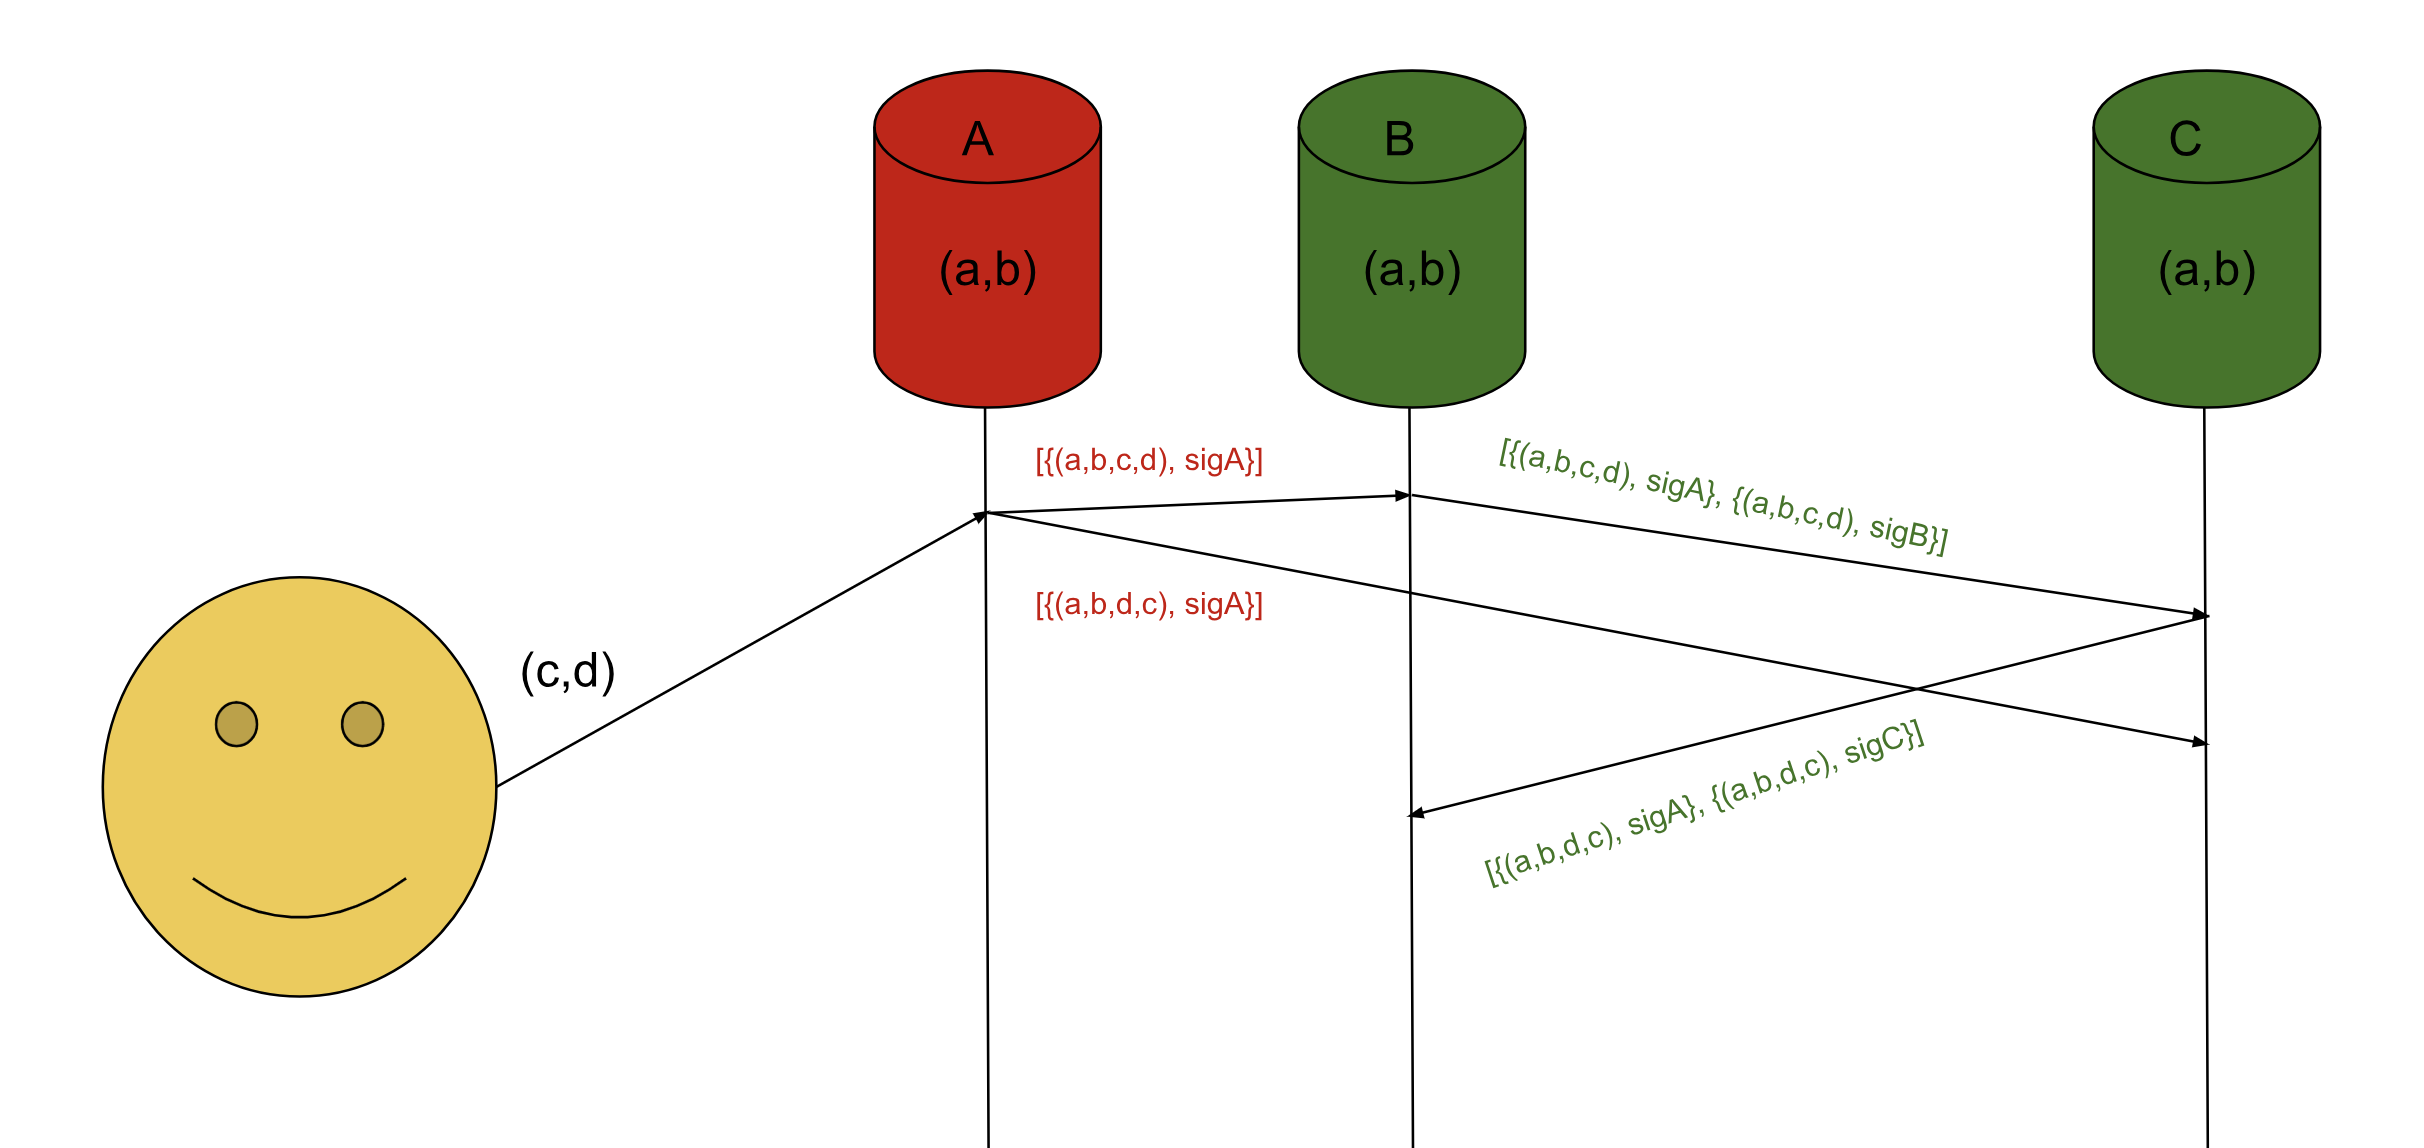
\includegraphics[width=\fscale{0.76}]{byz_faults.png}
	\caption{Byzantine fault detection during Paxos. Replica A sending conflicting messages is detected by B and C}
	\label{fig:byz_faults}
\end{figure}

\subsubsection{Sharding}
\textsf{Picolo} automatically partitions data into multiple shards when it grows too big for any one replica. Each shard consists of a set of key ranges (typically 64MB). A \textsf{key range} is the smallest atomic unit that is replicated aka governed by a paxos group. It is also the smallest unit of movement when data from one replica needs to be sharded into distinct replica sets. The process of sharding is a well studied problem in databases and implementations can be readily found, so we omit a detailed discussion here. 

\subsection{External consistency, Hybrid time \& Distributed transactions} \label{sec:hybrid_time}
Intuitively, external consistency property \cite{External_Consistency} of a distributed system guarantees that the state changes seen by it are exactly in the order applied to it by an external actor. It is the strongest form of consistency a distributed database system can offer and is notoriously hard to achieve in a system with asynchronous network links. Google's Spanner \cite{spanner} achieves this by using the TrueTime api which exposes clock uncertainty as an interval. Every transaction in Spanner has a TrueTime timestamp that indicates its time of entry into the system. Maximum clock uncertainty guaranteed by Truetime is 7ms (due to datacenter latencies); which means by making every transaction wait for 7ms before committing, Spanner can guarantee their total ordering system wide. While these low \textit{commit-wait} latencies (7ms) made possible by state of the art datacenters work fine for Spanner, a decentralized network like \textsf{Picolo} has no such luxuries and needs a new trick.
\subsubsection{Using timestamps}
\textsf{Picolo} uses hybrid time \cite{hybrid_time} - a combination of physical clocks and logical clocks for timestamping. Each node is assumed to provide an accurate enough physical timestamp by running a daemon process that syncs time with NTP stratum 1 servers like Google's external NTP service. If a node's clock is off by more than 500ms from the average of its paxos group, \textsf{Picolo} automatically kills it and finds a replacement. The logical clock is simply a monotonically increasing number appended to the physical time; so its possible to do a simple lexicographic comparison to determine relative order. For each write transaction, $\textsf{leader}_\textsf{view}$ assigns a hybrid timestamp to it before proposing it to replicas. So when two requests r1 followed by r2 hit the same paxos group and pass by $\textsf{leader}_\textsf{view}$, all the replicas are guaranteed to commit requests in the same order irrespective of the order in which they are received. For transactions that span multiple paxos groups, a coordinator (one of the $\textsf{leader}_\textsf{view}$ of individual paxos groups) is elected to perform a \textsf{2 phase commit (2PC)} with other leaders. In the \textsf{prepare} phase of 2PC, each leader acquires locks for its corresponding group and replies with its current timestamp. The coordinator then selects the highest timestamp of all the replies and uses it as the timestamp of the transaction during \textsf{apply} phase. This timestamp is also sent back to the initiator of the transaction so that it can pass it to a subsequent causally related transaction (if any). In the case where this propagation is not possible, external consistency cannot be guaranteed and application developers need to employ the commit wait strategy used by Spanner if desired, although at a performance expense.
\subsubsection{MVCC}
Multi version concurrency control (MVCC) is the practice of storing multiple versions of the same data. In \textsf{Picolo}, each record is uniquely identified by a timestamped key. So keys that differ only by their timestamps represent different versions of the same data. By keeping these different versions, \textsf{Picolo} offers such features as lock-free reads, time travel reads and snapshot isolation. Clients executing read transactions therefore need not acquire any locks since any concurrent writes on the same record have a newer timestamp and won't affect its older timestamped value. Records can also be fetched from the past by specifically executing a read transaction with an older timestamp. For writes however, a lock needs to be acquired on the key being modified. Lock status of keys is stored in a lock table and transactions that mutate data need to check whether the key/range of keys they try to operate on is already present in the lock table, in which case they need to wait. Else, they create an entry in the lock table (thereby acquiring the lock) before proceeding. Similarly, for writes spanning multiple paxos groups, one of the $\textsf{leader}_\textsf{view}$'s is chosen as the coordinator of a \textsf{2PL} (two phase locking) process that facilitates the locking of keys/key ranges of each group by its respective leader.

\subsection{Data in web 3.0}
Our long term goal for \textsf{Picolo} is to make it \textit{the} data network for web 3.0 (\cref{sect:applications}). Data in the new web will be solely controlled by data owners and resides in a single shared network. To support such a network, following capabilities must be built:
\subsubsection{Distributed query processing} \label{sec:dynamic_cluster}
A web 3.0 data network needs to have the capability to execute queries across $all$ nodes in the network in response to a client request. Since nodes will have vastly differing schemas, effective mechanisms for searching and query proessing \cite{query_reformulation, query_processing1, query_processing2} are needed. High level architecture of a \textsf{Picolo} node is depicted in \figref{fig:node_arch}.
\begin{figure}[h!] \centering
	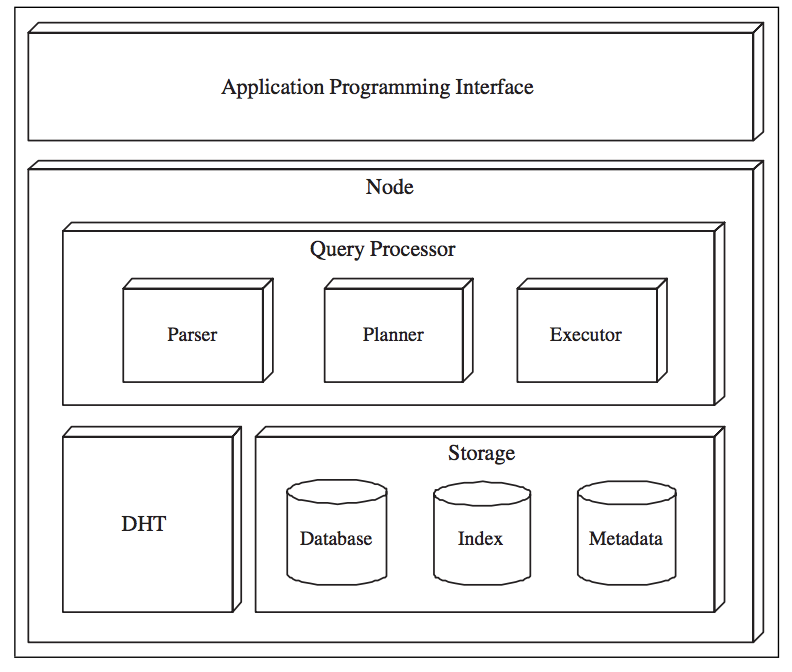
\includegraphics[width=\fscale{0.76}]{node_arch.png}
	\caption{A \textsf{Picolo} node}
	\label{fig:node_arch}
\end{figure}
The schema dictionary depicted in the figure contains metadata to be exposed to the world. Nodes that wish to keep data private should not export the data's metadata to the schema dictionary. Suppose there is a table called \textsf{users} with four columns: \textsf{username}, \textsf{firstname}, \textsf{lastname} and \textsf{email}. The exported metadata entry might look like:
\begin{center}
	\begin{tabular}{| c | c |} 
		\hline
		Entity & Keywords \\ [0.5ex] 
		\hline
		\textsf{users} & user, people, customer, profile\\ 
		\hline
		\textsf{name} & name \\
		\hline
		\textsf{firstname} & fn, {f\_name}, {first\_name} \\
		\hline
		\textsf{lastname} & ln, {l\_name}, {last\_name} \\
		\hline
		\textsf{email} & id, contact \\ [1ex] 
		\hline
	\end{tabular}
\end{center}
When a query is posed to any node in the system, the node first tries to fulfill it with a local query before passing it along to its neighbors. Remember, nodes in the system host data with heterogeneous schemas. Hence the keywords are used to find semantically similar data by assisting in query reformulations.
\newline\newline
\textbf{Dynamic clustering}:
Semantic proximity metrics \cite{PeerDB} and clustering techniques \cite{dynamic_clustering} can be used to find nodes hosting semantically similar schemas. Overtime, these nodes are discovered and are clustered together for better query performance by reducing the number of network hops required.

\subsubsection{Data sovereignty} \label{sec:access_control}
\textsf{Picolo} supports two different schema types: \textit{application controlled} and \textit{user controlled}. Applications can use user controlled schemas to put users in absolute control of data and better comply with regulations like GDPR. For example, a decentralized twitter may  want users to have control over their tweets. Users can use any third party client or \textsf{Picolo}'s official clients to interact with their tweets, effectively rendering the decentralized twitter just another client to the data albeit with better features. \newline\newline
When semantics don't allow to put user in control of data, application controlled schemas can be used. An example here would be a decentralized ticketing application where users should not be given fine grained control to selectively delete data about which tickets they bought.
\newline\newline
\textbf{Access control}:
Applications and users may want to share data with other parties but may wish to impose access controls. There are a few ways of achieving this including building an API on top of the data or using proxy re-encryption techniques. In \cite{ac_p2p_db}, a secret sharing scheme is used instead, where a party given access to encrypted data collects key shares from key holders, reconstructs the key and decrypts data for further use. Acces rules can be defined by a SQL like declarative language at any granularity desired like at the level of a single row or a cell. An example row level granularity rule looks like:\newline \newline
\texttt{SELECT  * \newline FROM users \newline WHERE email=foo@bar.com \newline NODE (SELECT nodeId FROM nodes WHERE domain=application)} \newline \newline
An example value level (only username is given access to) granularity rule looks like:\newline \newline
\texttt{ SELECT username \newline FROM users \newline WHERE email=foo@bar.com \newline NODE (SELECT nodeId FROM nodes)}\newline\newline
Here \texttt{NODE} is a new SQL clause that identifies nodes/actors in the network that have access to the data covered by the rule. Each access rule creates an ecrypted block of data. When there are overlapping rules, multiple encrypted blocks are created with associated keys. The scheme also supports updates to rules - however updates cause data re-encryption and key re-distribution. 

\subsubsection{Role of encryption}
Attribute based encryption (\textsf{ABE}) \cite{abe} was first described by Goyal et.al as a way to achieve fine grained access control on data stored with a third party. It allows attaching policies or access structures to cipher texts and allows decrypting them only if the decryption key has attributes that satisfy the access structure. As an example, in a patient-disease database, a policy could be to allow to only decrypt records where the disease is flu and only keys with the attribute \textit{flu} would be able to decrypt them. \textsf{ABE} comes in two forms: ciphertext-policy ABE (\textsf{CP-ABE}) and key-policy ABE (\textsf{KP-ABE}). In \textsf{CP-ABE}, policies are attached to ciphertexts and attributes are attached to keys whereas in \textsf{KP-ABE}, policies are attached to keys and ciphertexts are labelled with attributes. While these techniques sound promising, there don't seem to be many practical implementations of them in databases. Sieve \cite{sieve} uses \textsf{KP-ABE} to protect user data stored in files with a cloud storage provider. It uses an hybrid encryption scheme where data itself is ecnrypted using a symmetric key and metadata related to the file including its location and the symmetric key is encrypted with \textsf{KP-ABE}. A client first gets the metadata, decrypts it using a key which has a corresponding policy, downloads the file and decrypts it locally with the symmetric key. A similar technique is used in \cite{PPEHR}. The \textsf{ABE} schemes used in either of these systems seem to be secure only under a \textsf{selective-set} model which  may not be sufficient in all adversarial scenarios. Moreover, key revocation in Sieve requires re-encrypting data which may not scale well while in \cite{PPEHR}, the effectiveness of key revocation is not discussed in detail.
\newline\newline
Another body of research focuses on \textsf{ABE} schemes that are \textsf{CCA2} secure. In \cite{cca2_abe1} a \textsf{CCA2} secure \textsf{KP-ABE} scheme is proposed which is based on a \textsf{large universe} construction of another \textsf{KP-ABE} scheme. They overcome the limitations of the underlying scheme by adding a dummy on-the-fly attribute to the decryption procedure which is obtained by running a temporary message through a \textsf{chameleon hash} function. In \cite{cca2_abe2}, authors describe a scheme that is adaptively secure under the complexity assumptions of 3-prime subgroup decision problem. Their scheme allows dynamic update of policies tending itself suitable for practical use cases. But similar to Sieve, the data needs to be re-encrypted by the storage provider (albeit without sacrificing confidentiality). EASiER \cite{easier} is a system that allows for dynamic policy update without the need for data re-encryption. It uses a minimally trusted proxy that faciliates efficient access revocation and can be used in constructing practical systems that use \textsf{ABE} for access control.
\newline\newline
\textsf{Picolo} is the first system that uses \textsf{ABE} for fine-grained access control in a distributed database. It allows data owners to set access rules via the declarative language above and uses a \textsf{CCA2} secure \textsf{ABE} scheme with proxy assisted revocation. \textsf{Picolo}'s construction will be more comprehensively detailed in an upcoming paper.




\section{Random stuff}
\begin{table}[h]
\centering
\begin{tabular}{l l l}
\hline
\textbf{Treatments} & \textbf{Response 1} & \textbf{Response 2}\\
\hline
Treatment 1 & 0.0003262 & 0.562 \\
Treatment 2 & 0.0015681 & 0.910 \\
Treatment 3 & 0.0009271 & 0.296 \\
\hline
\end{tabular}
\caption{Table caption}
\end{table}


\begin{equation}
\label{eq:emc}
e = mc^2
\end{equation}

Some factors that affect prices of cryptos are listed below. These factors are by no means exhaustive but provide a
framework within which mechanisms to analyze them can be discussed. See the sub sections where some techniques are
presented. \cite{Picolo_Whitepaper}
Factors affecting the prices of crypto assets:

\section{Verifiable data structures, encryption, data sovereignty}

\section{Attacks on the system}


%-----------------------------------------------------------------------------
%  CONCLUSIONS
%-----------------------------------------------------------------------------
\section{Conclusion}
Initial implementations of AI algorithms that analyze structured and unstructured data are discussed. Unstructured data is analyzed in two steps: first, at a unit level and second as a sequence by feeding it to an LSTM. Structured data consisting of live feed from exchanges, current and past bets on the platform amongst others is represented as a game state where an independent decision making agent learns to take actions that maximize its game score. A method of determining payouts to platform users is discussed where they are determined by the magnitude as well as the category of contribution.


%-----------------------------------------------------------------------------
%  BIBLIOGRAPHY
%-----------------------------------------------------------------------------
\section{References}
\bibliography{./bib/picolo.bib}
\end{document}

%% The Appendices part is started with the command \appendix;
%% appendix sections are then done as normal sections
%% \appendix

%% \section{}
%% \label{}

%% References
%%
%% Following citation commands can be used in the body text:
%% Usage of \cite is as follows:
%%   \cite{key}          ==>>  [#]
%%   \cite[chap. 2]{key} ==>>  [#, chap. 2]
%%   \citet{key}         ==>>  Author [#]

%% References with bibTeX database:


%% Authors are advised to submit their bibtex database files. They are
%% requested to list a bibtex style file in the manuscript if they do
%% not want to use model1-num-names.bst.

%% References without bibTeX database:

% \begin{thebibliography}{00}

%% \bibitem must have the following form:
%%   \bibitem{key}...
%%
%% Example figure:
%%
%% \begin{figure}[h]
%% \centering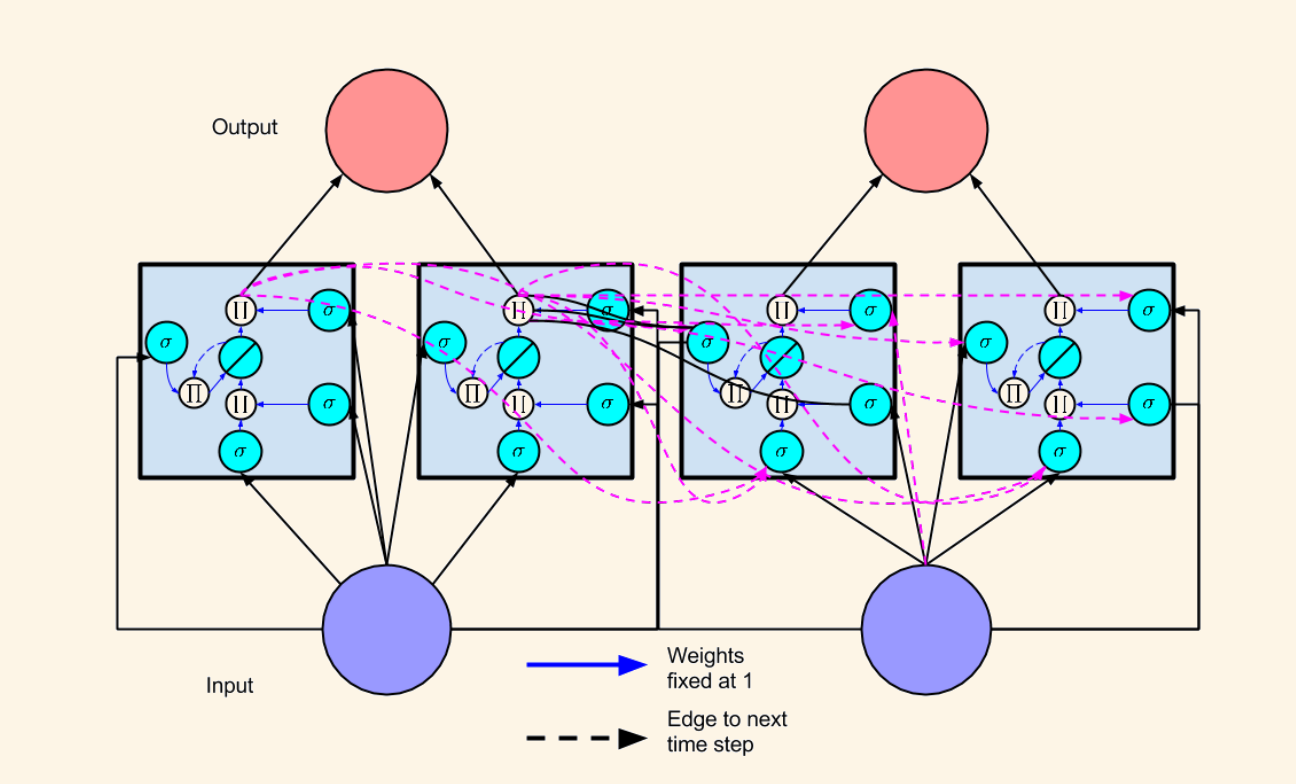
\includegraphics[width=0.4\linewidth]{placeholder.png}
%% \caption{Figure caption}
%% \end{figure}
%% 
% \bibitem{}

% \end{thebibliography}
